\section{Ranking Functions} \label{Sec:ranking}
In this section, we present our function ranking approach, which is used for selective variable and branch mutation.
%As it is shown in \figref{mutation}, 

 
\subsection{Ranking Functions for Variable Mutation}
\label{Sec:rankfunc-var}
%To rank functions for selective \emph{variable} mutation, we propose a new metric called $FunctionRank$. 

%
%In order to detect critical functions, that are more likely to exhibit severe bugs,
In order to rank and select functions for  variable mutation generation,  we propose a new metric called $FunctionRank$, which is based on $PageRank$  \cite{brin:cnis98}, but takes dynamic function calls into account. As such, $FunctionRank$ measures the relative importance of each function at runtime. %We compute $FunctionRank$ on the call graph of the application. 
To calculate this metric, we use a function call graph inferred from a combination of static and dynamic analysis (line 6 in \algref{mutationAlgo}). Our insight is that the more a function is used, the higher its impact will be on the application's behaviour. As such, we assign functions that are highly ranked, a higher selection probability for mutation.

\headbf{Function Call Graph} \label{Sec:functionCallGraph}
To create a function call graph, we use dynamic as well as static analysis.
We instrument the application to record the callee functions per call, which are  encountered during program execution.
However, the obtained dynamic call graph may be incomplete due to the presence of uncovered functions during the program execution.
Therefore, to achieve a more complete function call graph, we further infer the static call graph through static analysis. 
We detect the following types of function calls in our static analysis of the application's code:

\begin{enumerate}
 \item Regular function calls \eg~\code{foo()};
 \item Method calls \eg~\code{obj.foo()};
 \item Constructors \eg~\code{new foo()};
 \item Function handlers \eg~\code{e.click(foo)};
 \item Anonymous functions called by either a variable or an object property where the anonymous function is saved.
\end{enumerate}

We enhance our dynamically inferred call graph of the executed functions by merging the graph with the statically obtained call graph containing uncovered functions. 
Note that constructing function call graph for the \javascript applications using static analysis is often unsound due to highly dynamic nature of the \javascript language. In \javascript functions can be called through dynamic property access (e.g., \code{array[func]}). They can be stored in object properties with different names, and properties can be dynamically added or removed. Moreover, \javascript functions are first class meaning that they can be passed as parameters. While static program analysis cannot reason about such dynamic function calls in \javascript applications, relying on pure dynamic analysis can also lead to an incomplete call graph because of the unexecuted functions that are part of the uncovered code at run-time. Therefore, in our approach we choose to first construct our function call graph based on dynamic information obtained during the execution, and then make use of static analysis for those functions that are remained uncovered during the execution. 
%\karthik{So do we calculate the union of the two graphs ? How is this more accurate than just the static graph ?}

\headbf{Dynamic Call Frequencies} \label{Sec:dynamicCallFreq}
While the caller-callee edges in the call graph are constructed through static analysis of the application's code, the call frequency for each function is inferred dynamically from the execution traces (line 3 in \algref{mutationAlgo}).
The call graph also contains a mock node, called $main$ function, which represents the entire code block in the global scope, \ie global variables and statements that are not part of any particular function.
The $main$ node does not correspond to any function in the program.
In addition, function event handlers, which are executed as a result of triggering an event, are linked to the $main$ node in our dynamic call graph.

\IncMargin{0.5em}
\begin{algorithm}[t]
{\scriptsize
\SetKwInOut{Input}{input}\SetKwInOut{Output}{output}
\Input{A Web application $App$, the maximum number of variable mutations $MaxVarMut$ and branch mutations $MaxBrnMut$}
\Output{The mutated versions of application \textit{Mutants}}
\BlankLine
\nl \textit{App} $\leftarrow \textsc{Instrument}(App)$ \\
\Begin {
\nl \textit{trace} $\leftarrow \textsc{CollectTrace}(App)$ \\
\nl $\{callFrq_{f_{i,j}}, varUsgFrq_{f_{i}}, invars_{f_{i}}\}$ $\leftarrow \textsc{GetRequiredInfo}(\textit{trace})$\\
\nl $l=m=0$\\
\nl \While {$l<MaxVarMut$}{
\nl 	$\{FR(f_i)_{i=0}^n\}$ $\leftarrow \textsc{FunctionRank}(callGraph, callFrq_{f_{i,j}})$\\
\nl 	\textit{mutF} $\leftarrow \textsc{SelectFunc}(\big(FR(f_i)\big)_{i=0}^n)$\\
\nl 	$\alpha$ $\leftarrow$ $\frac{1}{1-ReadVar_{f_{i}}}$\\
\nl 	$candidVars_{mutF}$ $\leftarrow invars_{mutF} \cup \{v_i|varUsgFrq_{mutF}(v_i)>\alpha\}$\\
\nl 	$\{pr(v_i\in candidVars_{mutF})\}$ $\leftarrow \frac{1}{|candidVars_{mutF}|}$\\
\nl 	\textit{mutVar} $\leftarrow \textsc{SelectVar}(candidVars_{mutF}, pr(v_i))$ \\
\nl 	$mutant_l \leftarrow \textsc{VariableMutation}(mutF,mutVar,varMutOps)$\\ 	
\nl 	$l++$\\
}
\nl \textit{varMutants} $\leftarrow \bigcup mutant_{l=1}^{MaxVarMut}$\\
\nl \While {$m<MaxBrnMut$}{
\nl 	$\{pr(f_i)_{i=0}^n\}$ $\leftarrow \frac{fcc(f_i) \times FR(f_i)}{\sum _{j=1}^{n} fcc(f_i) \times FR(f_i)}$\\
\nl 	\textit{mutF} $\leftarrow \textsc{SelectFunc}(\big(pr(f_i)\big)_{i=0}^n)$\\  
\nl 	\textit{mutBrn} $\leftarrow \textsc{SelectRandomBrn}(mutF)$ \\
\nl 	$mutant_m \leftarrow \textsc{BranchMutation}(mutBrn,brnMutOps)$\\
\nl 	$m++$\\
}
\nl \textit{brnMutants} $\leftarrow \bigcup mutant_{m=1}^{MaxBrnMut}$\\
\nl \textit{Mutants} $\leftarrow varMutants \cup brnMutants$\\
\nl return \textit{Mutants}
}
\caption{Guided Mutation Algorithm.}
\label{Alg:mutationAlgo}
}
\end{algorithm}
%\DecMargin{lem}

\headbf{The FunctionRank Metric} 
%\label{Sec:functionRankMetric} \ali{this is not a section so labels won't work}
The original $PageRank$ algorithm \cite{brin:cnis98} assumes that for a given vertex, 
the probability of following all outgoing edges is identical, and hence
all edges have the same weight. For $FunctionRank$, 
we instead apply edge weights proportional to the dynamic call frequencies of the functions.  % obtained from  execution traces. %(by using a relaxed form of the original formula). 
%However, the $PageRank$ formula requires that
%the weights on the outgoing edges sum to 1. 
%Therefore, we need to normalize the edge weights from 
%each function in our formula. 

Let $l(f_{j},f_{i})$ be the weight assigned to 
edge $(f_{j},f_{i})$, in which function $i$ is called by function $j$. 
We compute $l$ by measuring the frequency of function $j$ calling $i$ 
during the execution.  We assign a frequency of 1 to edges directing to unexecuted functions.
%We consider the number of times that function $i$ calls an unexecuted function during the application's run is equal to one. 
The $FunctionRank$ metric is calculated as:

\begin{equation}
FR(f_i)=\sum _{j\in M(f_i)} {FR(f_j)\times l(f_j,f_i)},
\label{functionRankFormula}
\end{equation}
where, $FR(f_i)$ is the $FunctionRank$ value of function $i$, $l(f_j,f_i)$ is
the frequency of calls from function $j$ to $i$, and $M(f_i)$ is the set of
functions that call function $i$%., and $n$ is the total number of functions.

The initial $PageRank$ metric requires 
the sum of weights on the outgoing edges to be 1.
Therefore, to solve equation \ref{functionRankFormula}, we need to normalize the edge weights from 
each function in our formula such that for each $i$,
$\sum _{j=1}^{n} {l(f_i,f_j)}=1$.   
To preserve the impact value of call frequencies on edges when compared globally in the graph,
we normalize $l(f_i,f_j)$ over the sum of weights on all edges. Since outgoing edges from
function $f_i$ should sum to 1, an extra node called $fakeNode$ is added to the graph. Note that the extra $fakeNode$ is different from the mock $main$ node added earlier. $fakeNode$ contains an incoming edge from $f_i$, where:
%\karthik{We should make it clear that the fakeNode is different from the mock node added earlier}

\begin{equation}
 l(f_i,fakeNode)=1-\sum _{j=1}^{n} {l(f_i,f_j)}
 \end{equation}

Functions with no calls are also linked to the $fakeNode$ through an outgoing edge with weight 1.

A recursive function is represented by a self-loop to the recursive node in the function call graph.
The original $PageRank$ does not allow for self-loop nodes (\ie a web page with a link to itself).
Self-loop to a node infinitely increases its rank without changing the relative rank of the other
nodes. Therefore, such nodes are disregarded in the original $PageRank$ formula. 
However, recursive functions are inherently important as they are error-prone and difficult to debug, and they can easily propagate a fault into higher level functions. To incorporate recursive functions in our analysis, we break the self-loop to a recursive function $Recf_i$ by replacing the function with nodes $f_i$ and $f_{ci}$ in the function call graph. We further add an edge $l(f_i,f_{ci})$, where $l$ is the call frequency associated with the recursive call. 
All functions that are called by $Recf_i$ will get an incoming edge from the added node $f_{ci}$.  
This way,  all the functions called by $Recf_i$ are now linked to $f_{ci}$ (and indirectly linked to $f_i$).
After the $FunctionRank$ metric is computed over all functions, we assign the new $FunctionRank$ value of the recursive node as follows: 
$FR(Recf_i)=FR(f_i)+FR(f_{ci})$, where $FR(Recf_i)$ is the new $FunctionRank$ value assigned to the recursive function $Recf_i$. %\ali{I don't understand this previous paragraph. We need a better explanation of what we are doing and why we are doing it.}

\begin{figure*} [tp]
\centering
\subfloat[Call graph with call numbers.]{\label{Fig:origGraph}
       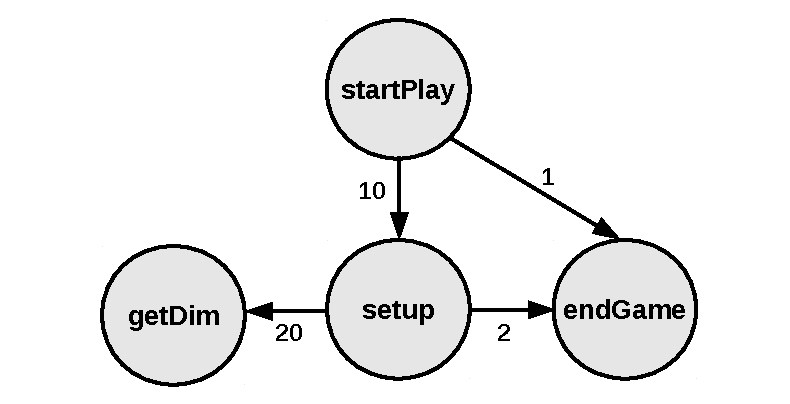
\includegraphics[width=.4\textwidth]{fig/exampleGraph0}}
\subfloat[Call graph with call frequencies.]{\label{Fig:modifGraph}
       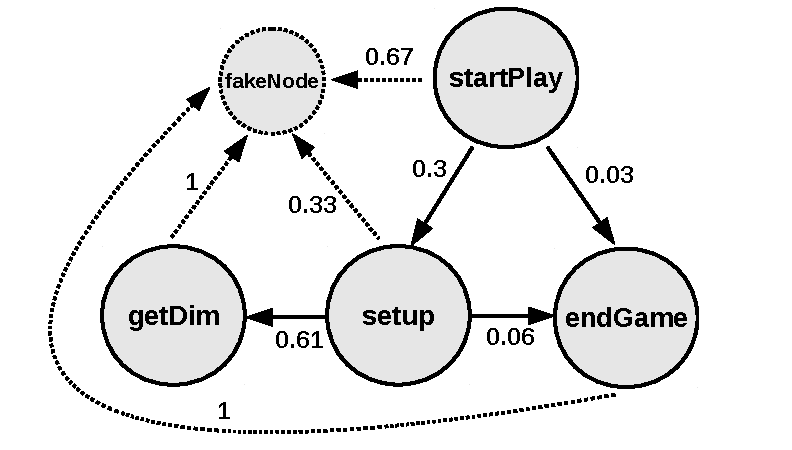
\includegraphics[width=.4\textwidth]{fig/exampleGraph}}
\vspace{0.2in}             
\caption{Call graph of the running example.}
\label{Fig:exampleGraph}
\end{figure*}
 
%\begin{figure}
%\centering
%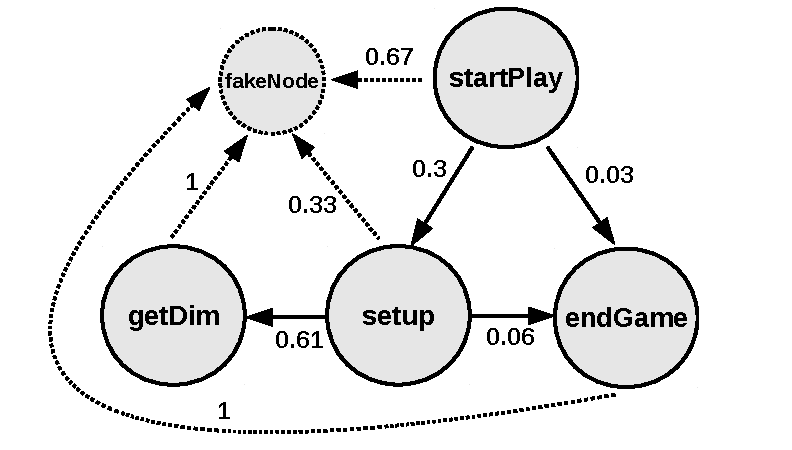
\includegraphics[width=0.8\hsize]{fig/exampleGraph}
%\vspace{0.15in} 
%\mycaption{Call graph of the running example.}
%\label{Fig:exampleGraph}
%\vspace{-0.1in} 
We initially assign equal $FunctionRank$ values to all nodes in \ref{functionRankFormula}.%\end{figure}
The calculation of $FunctionRank$ is performed recursively, %\ali{isn't it recursivly?},
until the values converge. 
Thus,  the $FunctionRank$ of a function $i$ depends on:

\begin{enumerate}
\item the number of functions that call $i$;
\item the $FunctionRank$ values of the functions that call $i$ (incoming edges);
\item the number of dynamic calls to $i$.
\end{enumerate}

Hence, a function that is called by several functions with high $FunctionRank$s
and high call frequencies receives a high $FunctionRank$ itself.

At the end of the process, the extra function $fakeNode$ is removed and the $FunctionRank$ value of all other functions is multiplied by $\frac{1}{1-FR_{fakeNode}}$, where $FR_{fakeNode}$ is the calculated 
$FunctionRank$ of $fakeNode$. 

Overall, our approach assigns each function a $FunctionRank$  value between 0 and 1.
These values are used to rank and select functions for variable mutation (lines 6-7 in \algref{mutationAlgo}). 
The higher the $FunctionRank$ value of a given function, the more 
likely it is to be selected for mutation. 

\figref{exampleGraph} depicts the function call graph obtained from our running example (\figref{example}). The labels on the edges of \figref{origGraph} show the
number of calls to each function in the graph. \figref{modifGraph} shows the modified graph with the extra node $fakeNode$ added to compute the normalized function call frequency  values.
%The labels on the edges of \figref{modifGraph} are edge weights calculated according to the function call frequency. 
In our example, assuming that the number of \code{div} elements is 20 (line 3 in \figref{example}), \code{setup} will be called 20 times and \code{endGame} will be called once (lines 4 and 6). Now, assume that the number of DOM elements with the class name specified as the input to function \code{setup} varies each time \code{setup} is called (line 10) such that two elements have a length of zero and the total length of the rest is  20. Then, function \code{endGame} is called twice (in line 12) when the length of such elements is zero, and \code{getDim} is called 20 times in total (line 14). Therefore, the call frequencies of functions \code{setup} and
\code{endGame} become 0.3 and 0.03 respectively when they are called by \code{startPlay} in lines 4 and 6.
Similarly, the call frequencies of \code{getDim} and \code{endGame} become 0.61
and 0.06, respectively, when called by \code{setup}. 

Note that if the weight on an outgoing edge of a given function is simply normalized over the sum of the weights on all the outgoing edges of that function, then the call frequencies  
for both \code{setup} and \code{getDim} become 0.91 when they are called by \code{startPlay} and \code{setup}, respectively. However, as shown in \figref{origGraph} the number of times that function \code{getDim} is called is twice that of \code{setup}. To obtain a realistic normalization, we have introduced the $fakeNode$, as shown in \figref{modifGraph}.
 
%Using equation \ref{functionRankFormula}, we are able to calculate $FunctionRank$ values associated with each of the functions in the graph shown in \figref{modifGraph}. 
\tabref{fr-pr-table} shows the computed 
$FunctionRank$ values, using equation \ref{functionRankFormula}, for each function of the running example. The values are presented as percentages. \code{getDim} achieves the highest $FunctionRank$ because of the relatively high values of both the incoming edge weight (where \code{getDim} is called by \code{setup} in line 14 in \figref{example}), and the $FunctionRank$ of its caller node, \code{setup}.
These ranking values are used as probability values for selecting a function for mutation. 

To illustrate the advantage of $FunctionRank$, we show the same calculation using the traditional $PageRank$ metric, i.e., without considering dynamic edge weights. As shown in \tabref{fr-pr-table}, \code{endGame} obtains the highest ranking using $PageRank$. However, this function has not been used extensively during the application execution, and hence has only limited impact on the behaviour of the application. 
In contrast, when $FunctionRank$ is used, \code{endGame} falls to the third place, and is hence less likely to be chosen for mutation. 

%$FR(\code{endGame})<\frac{1}{2}FR(\code{getDim})$. Thus, the probability of choosing
%\code{getDim} for mutation is considerably higher than \code{endGame}. 

\begin{table}
%\vspace{5pt}
        \caption{Computed $FunctionRank$ and $PageRank$ for the running example.}
{\scriptsize
   
       \begin{center}
      %  \subtable[Experimental subjects and the corresponding exploration data]
            {
          \begin{tabular}{l|c|c} \hline
\thead{Function Name} & \thead{FunctionRank (\%)} & \thead{PageRank (\%)} \\  \hline \hline

  \code{getDim} & 34.5 & 27.0 \\ \hline
  \code{setup} & 25.0 & 23.0 \\ \hline
  \code{endGame} & 21.3 & 34.6 \\ \hline
  \code{startPlay} & 19.2 & 15.4 \\ \hline

\hline \end{tabular}\centering
            }

\label{Table:fr-pr-table}
\end{center}
}  
\vspace{-0.1in} 
\end{table}

\subsection{Ranking Functions for Branch Mutation}
\label{Sec:funcrank-branch}
%In addition to calculating $FunctionRank$ based on the dynamic analysis of application, we also take the structural complexity of functions into account in order to mutate branch statements of the program. 
To rank functions for \emph{branch} mutation, in addition to the $FunctionRank$, we take the cyclomatic complexity of the functions into account (lines 16--17 in \algref{mutationAlgo}).

%As mentioned before, we use the cyclomatic complexity of  a function in addition to its $FunctionRank$ to select functions for branch mutation (lines 16-17 in \algref{mutationAlgo}). 
%Cyclomatic complexity is one of the widely used metrics to measure the structural complexity of a function \cite{mccabe:tse76}.
The cyclomatic complexity measures the number of linearly independent paths through a program's source code~\cite{mccabe:tse76}. By using this metric, we aim to 
concentrate the branch mutation testing effort on the functions that are error-prone and harder to test.

We measure the cyclomatic complexity frequency of each function through static analysis of the code. Let $fcc(f_i)$ be the cyclomatic complexity frequency measured for function $f_i$, then $fcc(f_i)=\frac{cc(f_i)}{\sum _{j=1}^{n} cc(f_j)}$,  
where $cc(f_i)$ is the cyclomatic complexity of function $f_i$, given that the total number of functions in the application
is equal to $n$.

We compute the probability of choosing a function $f_i$ for branch mutation using the previously measured $FunctionRank$ ($FR(f_i)$) as well as the cyclomatic complexity frequency ($fcc(f_i)$). Let $p(f_i)$ be the probability of selecting a function $f_i$ for branch mutation, then:

\begin{equation}
p(f_i)= \frac{fcc(f_i) \times FR(f_i)}{\sum _{j=1}^{n} fcc(f_j) \times FR(f_j)},
\label{fr-cc-formula}
\end{equation} 
where $fcc(f_i)$ is the cyclomatic complexity frequency measured for function $f_i$, and $n$ is the total number of  functions.

\begin{table}
%\vspace{5pt}
        \caption{Ranking functions for branch mutation (running example).}
{\scriptsize
   
       \begin{center}
      %  \subtable[Experimental subjects and the corresponding exploration data]
            {
          \begin{tabular}{l|c|c|c} \hline
\thead{Function Name} & \thead{cc} & \thead{fcc} & \thead{Selection Probability ($p$)} \\  \hline \hline

  getDim & 4 & 0.4 & 0.51\\ \hline
  setup & 3 & 0.3 & 0.27\\ \hline
  startPlay & 2 & 0.2 & 0.14\\ \hline
  endGame & 1 & 0.1 & 0.08\\ \hline


 	
\hline \end{tabular}\centering
            }

\label{Table:cycloMultFr-table}
\end{center}
}  
\vspace{-0.1in} 
\end{table}
\tabref{cycloMultFr-table} shows the cyclomatic complexity, the frequency, and the function selection
probability measured for each function in our example (\figref{example}). The probabilities are obtained using equation \ref{fr-cc-formula}.
As shown in the table, \code{getDim} achieves the highest selection probability as both its $FunctionRank$ and cyclomatic complexity
are high.

